\chapter{Problem}
\label{ch:Problem}

\section{Problem statement}

In this project we proposed to develop a simulation software package that permits analysis of electromagnetic (EM) wave propagation, in the context of Photonic Crystal (PC) defects modelling and design.

%Problem statement will herein be addressed as the goal of the project.
% Being so it is an abstraction of what has to be accomplished.
% Objectives, which are to be addressed next reffer to the specifics of the problem statment
% It is very likely that the problem statement and a general objective be confused, actiually I do. Maybe they are the same. I address this confusion here making the general objective a bit more implementation-oriented.
\section{Objectives }
The following were the objectives as stated in the project proposal document:
\subsection{General objectives}
\begin{itemize}
\item Build a software platform capable of simulating   electromagnetic field propagation in perfect PC and also in PC with defects such as cavities and inclusions.
\item The platform architecture must be structured in a way that facilitates future upgrading, possible optimization schemes, and integration with other kinds of simulations like confinement of electrons in potential wells and crystals. 
\end{itemize}

% Objectives must be S.M.A.R.T:
% Specific, Measurable, Achievable, Relevant and Time-bound.%


\subsubsection{Specific objectives}
\begin{enumerate}
\item  Apprehend the theory behind EM fields and its applications in photonics. Particularly: 
\begin{enumerate}
	 \item general overview of computational methods in electromagnetism and deeper understanding of methods that fit the problem statement.
	 \item Photonic crystals and the mathematical tools for modeling periodicity, as well as 
	 \item technological applications of defects in photonic crystals and common case studies. 
\end{enumerate}

\item Define a set of implementation requirements and constraints, in terms of the numerical method, and expected functionality.  

\item Implement algorithms to solve problems that relate to technological applications studied in the appropriation stage. 
	\begin{enumerate}
	\item Solve simple scalar-static 2D problems
	\item Implement vector field solver for stationary non periodic conditions (this may qualify as spectral solution or not)
	\item Vector field solutions for time dependent problems
	\item Introduce periodic conditions
	\end{enumerate}
	
\item Document and share the results of the simulations making an analysis of the relevance and feasibility of the platform. 
\end{enumerate}

\section{Justification}

%Materials are important,
Most of the artificial environment we as a society have built to live in, is in one way or another a consequence of our ability to understand and transform materials present in nature. This understanding is so important that human history studies have come to address cultural stages of our evolution from: the Stone Age through Bronce Age, as the materials we used to overcome survival challenges \cite{Joannopoulos2008}. Even in recent years, extraordinary changes in the way we evolve as a species can be attributed to achievements only possible by improvements on our understanding of material properties. Take for example the paradigm change caused by the discovery of electronic properties of materials such as semiconductors \cite{Obayya2011}. And the ever growing stream of technological applications derived from it.
% Now that it has been stated that materials are important  I'll like to say that as discoveries in electronic properties of materials made a huge leap for humanity (towards somewhere), discoveries and study of optical properties of materials have the chance to become a new and equivalent paradigm change.
%Metamaterials can be generally defined as a class of ‘‘artificial’’ media, possessing extraordinary electromagnetic properties that cannot be found in natural ones. \cite{YangHao2009}.
%Metamaterials are a new class of ordered composites that exhibit exceptional properties not readily observed in nature. These properties arise from qualitatively new response functions that are: (1) not observed in the constituent materials and (2) result from the inclusion of artificially fabricated, extrinsic, low dimensional inhomogeneities. \cite{DARPA}.
% A metamaterial is a macroscopic composite of periodic or non-periodic structure, whose function is due to both the cellular architecture and the chemical composition. If the metamaterial is regarded as an effective medium, there is an aditional requirement that the cellular size is smaller than or equal to the the subwavelenght. \cite{TieJunCui2010}
% The core concept of metamaterial is to replace the molecules with man-made structures, viewed as “artificial atoms” on a scale much less than the relevant wavelength. In this way, the metamaterial can be described using a small number of effective parameters. In late 1960s, \cite{ZHang2010}.

The next frontier in the context of material science, relies in a level of understanding that allows us to not only use and transform materials, but to design them. This is the field of metamaterials, a field in which by means of manipulating the microscopical structure and geometry of a crystal-like solid, we can obtain macroscopic properties that are otherwise impossible to find in nature \cite{Engheta2006, Capoliono2009}. One of the sub domains of the metamaterials frontier is that of media capable of molding and manipulating electromagnetic waves. The ability to harness light has the prospect to support a new technological revolution of a scale similar to that of transistor revolution \cite{Joannopoulos2008}.
%In the words of Obayya 
%An enormous range of technological developments would become possible if we could engineer materials that respond to light waves over a desired range of frequecies by perfectly reflecting them, or allowing them to propagate only in certain directions, or confining them within a specified volume.
Advances in engineered optical materials will benefit the development of areas such as high speed computing, spectroscopy, laser engineering, biomedicine and quantum computing \cite{Obayya2011}. 
% Then Say something about photonic crystals and how they are cool. After that mention that preliminary study and design of photonic components is better in a simulation enviromnent.  Mainly because you dont have to build in order to test. Also because you can sistematically optimize \cite{H.Men2010}.
This project concerns about one candidate of optical metamaterial set known as photonic crystals, and particularly, the light guiding properties that arise when taking advantage of lattice cavities.
Photonic crystals are: 

\begin{quote}
\textit{``Artificially created periodic low-loss dielectric medium in which electromagnetic waves of certain frequencies cannot propagate \cite{GangBao1987}''}.  
\end{quote} 

Light in that certain frequency gap is virtually stopped because of periodicity of dielectric dispersers and the destructive interference that arises from it. This property is used in technical application for many forms of technological developments. For example Kärtner's et al. developed high resolution PC based Analogic-Digital (AD) conversion circuits \cite{F.X.Kaertner2006} that are showing all-optical circuits which outperform electronic based components. Telecommunications also benefit from technologies such as ultra low loss \href{http://en.wikipedia.org/wiki/Photonic-crystal_fiber}{photonic crystal fibers} \cite{A.M.Apetrei2005}. As well as low cost, and high definition spectroscopy technologies that take advantage of spectral selectivity in PCs; Pervez \cite{Pervez2010} has used a phenomenon called outcoupling to fabricate cheap PC based spectrometers. On the other hand, a lot of effort has been made to exploit the light confinement properties of PCs to make micro laser cavities and even single-photon sources. Theoretical background and numerical studies on spontaneous emission using microcavities in PCs has been undertaken by many researchers including works from Yablonovich and Vileneuve \cite{Yablonovich1987,Yablonovich1991,Villeneuve1996}. Experimental meassures of ultrafast nanocavity lasers was performed by Hatice \cite{Altug2006} in 2006, and Moore \cite{Moore2008} in 2008. Even state of the art quantum computing experiments are being possible by using PC based waveguides and cavities as shown by Wolters in \cite{Wolters2010}.

The nature of most PC application problems, is of such complexity that very often numerical tools are the only way of modeling new designs and performance. Figure \ref{fig:simulation_areas} shows some of the fields that benefit from electromagnetic numerical simulations as stated by Jin \cite{Jin2010}.  Computational methods such as: Plane Wave Expansion (PWE) \cite{StevenG.Johnson2001,Loaiza2011},  Finite Difference Time Domain (FDTD) \cite{A.M.Apetrei2005,Oskooi2009}, Method of Moments (MoM) or Boundary Element Method (BEM) and Finite Element Methods (FEM)\cite{Rodriguez2005,Masanori2001}, have had their share in the modeling of electromagnetic fields under many different scenarios. Every one of them having their own strengths and weaknesses in terms of: ease of implementation, precision, and computational resources.

\begin{figure}[h]
\centering
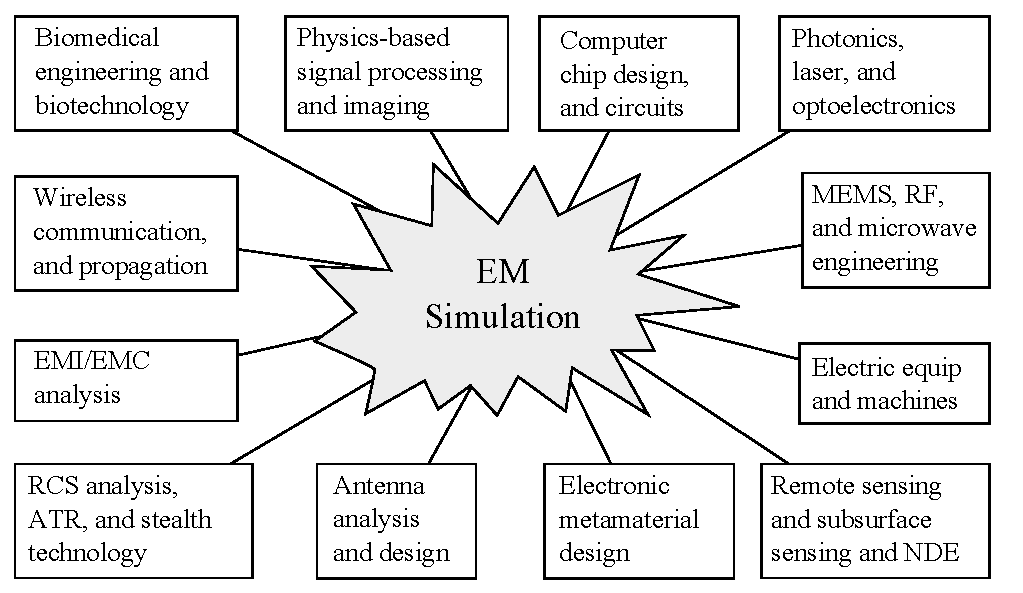
\includegraphics[scale=0.5]{./img/EM_simulation_applications.pdf}
\caption{Maxwell equations by the hand of numerical methods have the power to impact many scientific and technological areas. Taken from Jin et al \cite{Jin2010}}.
\label{fig:simulation_areas}
\end{figure}

In the context of Universidad EAFIT, and specifically of Engineering Physics, we see a growing research background in computational physics that goes from modeling seismic waves \cite{Guarin2012}, and resonant modes in musical instruments \cite{Rodriguez2012}; passing through quantum mechanics like relativistic phenomena in graphene \cite{Villegas2011}, and quantum potential wells and crystals \cite{Echeverri2011}; to finally address a computational module for digital holography and speckle \cite{Sierra2010}, and research on Plane Wave Methods for calculation of bandgap structures in photonic crystals \cite{Loaiza2011}. It can be stated that this trend in numerical methods applied to crystal-like materials has been embraced and supported by the Computational and Theoretical Physics Research Initiative of engineering physics students (\href{https://sites.google.com/site/fisicatyc/home}{SFTyC}). This work expands and continues the initiative towards strengthening undergraduate research and software development abilities. 


\pagebreak